% A report.pdf covering:

% Project design
% Installation & running instructions (pointing to requirements.txt or equivalent, in adherence to the dependencies form)
% Code structure — what each file/module does
% References/citations
% Optionally, a README as well. For the GitHub repo, ensure there is at least a minimal README.

%%%%%%%%%%%%%%%%%%%%%%%%%%%%%%%%%%%%%%%%%%%%%%%%%%%%%%%%%%%%%%%%%%%%%%%%%

% 8.3 Report (LaTeX)
% The report must include:
% A list of external libraries used and their purpose, with appropriate versions (see below)
% A description of all features implemented
% An explanation of how the three layers communicate, with reference to your code
% The format chosen for history.txt and why
% Hurdles faced and how you overcame them
% What you would do differently with 10 more hours
% Bibliography with references and links to external sources
% Write a suitable Makefile to compile the latex report

%%%%%%%%%%%%%%%%%%%%%%%%%%%%%%%%%%%%%%%%%%%%%%%%%%%%%%%%%%%%%%%%%%%%%%%%%

% Your submission must include a compiled report.pdf (12pt font, standard margins, 5–10 pages excluding figures/screenshots) along with source and makefile, structured as follows:

% External Libraries — List all external libraries/tools used and their purpose.

% Design & Architecture — Project-specific design and architectural decisions: how the system is structured, major components, and the reasoning behind key choices.

% Features Implemented — Description of all features you implemented.

% Directory Structure — A tree with one-line annotations per file/module.

% Installation & Setup — How to install dependencies and get the project running (requirements.txt or equivalent). Include Drive links for any large assets not bundled in the submission.

% Usage — How to run and interact with the project. Screenshots welcome.

% Retrospective — Challenges you faced, how you overcame them, and what you'd do differently given more time.

% References (optional) — Papers, resources, or links to external sources.


\documentclass[12pt]{article}
\usepackage[utf8]{inputenc}
\usepackage{subcaption}
\usepackage{amsmath}
\usepackage{amssymb}
\usepackage{hyperref}
\usepackage{titlesec}
\usepackage{xcolor}
\usepackage{fancyhdr}
\usepackage{graphicx}
\usepackage{multirow}
\usepackage{float}
\usepackage[rightcaption]{sidecap}
\usepackage{verbatim}
\usepackage[backend=bibtex]{biblatex}
\usepackage[a4paper, margin=1in]{geometry}
\hypersetup{
    colorlinks=true,
    linkcolor=blue,
    filecolor=magenta,      
    urlcolor=cyan,
}

\graphicspath{{report_images}}

\title{\textbf{CS108 Project Report \\ Snake Game}}
\author{
Vasu Vijay, Yash Meshiya \\ 25B1047, 25B1046 \\ \\
Department of Computer Science and Engineering \\
Indian Institute of Technology Bombay
}

\date{\today}

\begin{document}

\maketitle

\tableofcontents
\clearpage

\section{Introduction}
This project is to build snake game made with JS + HTML5 Canvas + Bootstrap 5, powered by a Flask API and a CLI admin tool (Bash) for leaderboard management.
This project is to build a snake game on a web page using JavaScript for handling logics, HTML5 Canvas for graphics and the use of CSS with Bootstrap 5.0 framework for responsive styling. The web app sends the records of all the games played to a backend server made using the Flask 3.1.0 library of Python 3.10, via a POST method. The backend then validates this record and saves it to a plaintext file. This plaintext file can be inspected and managed using an admin panel TUI built using a bash script.
% \section{Objectives}


\section{Libraries used}
A number of external and internal libraries were used in the project to either enhance functionality, design, code quality, or to implement critical features.\\
\subsection{Libraries used in bash}
\begin{itemize}
    \item \texttt{fold}: To wrap text around for different terminal window sizes
    \item \texttt{date}: To check validity and format of timestamp stored in \texttt{history.txt}
    \item \texttt{awk}: To handle history.txt for multiple uses, to handle file content line by line and print it in a formatted manner.
\end{itemize}

\subsection{Libraries used in python}
\begin{itemize}
    \item \textbf{Flask v3.1.0}: Flask was used to set up the web app's backend. It serves the web app to localhost (http://127.0.0.1:5000) and listens to fetch requests sent by JS on \texttt{/save\_score}. It also sends back a response indicating success/failure.
    \item \textbf{Standard libraries like: datetime, os, re}: \texttt{datetime} was used for validating the date and its format before saving. \texttt{re} was used for basic regex and \texttt{os} was used to traverse the project directory and add all sprite paths to data.js on server start.
\end{itemize}

\subsection{Libraries used in web app}
\begin{itemize}
    \item \textbf{Bootstrap v5.0}: Bootstrap was used to make all the modals which handles basic styling and functioning. It was also used to make the all the elements on the web page responsive and easy to code.
\end{itemize}

\section{Features}
\subsection{Web-based Snake Game}
\begin{enumerate}
    \item \underline{Start Menu}:
    The website has a menu which opens up on pageload in which the user can adjust basic settings before starting the game.\\
    Inside the modal menu, the user can enter their username, select a mode, and view the rules by clicking on the Rules button and opening the rules modal. After finishing this, they can proceed to the main game area by pressing Start Game.\\

    \item \underline{Basic game mechanics}:
    The web-based Snake Game includes all the essential gameplay mechanics required for a complete and functional classic snake experience. The snake moves on a grid-based board using keyboard controls, and fruits spawn randomly on the board, one at a time. Collision detection is implemented for both wall collisions and self-collisions, which trigger the game over condition.

    \item \underline{Fruits}:
    Multiple fruits have been implemented, and each produces a different effect on the snake's state when consumed. 
    \begin{itemize}
        \item \textbf{Carrot}: Consuming one carrot increases the score by 1.
        \item \textbf{Triple Carrot}: Consuming a Triple Carrot increases the score instantly by 3. Length updation is done tick by tick, increasing 1 unit length per game-tick.
        \item \textbf{Golden Apple}: Consuming a Golden Apple doesn't change but score, but it grants the snake invincibility, for a total of 30 game ticks. While invincible, the snake can not die. If it hits a wall, it will come out of the opposite edge, and if it hits itself, it will just slither over its body without dying. However, if the invincibility timer ends while the snake is in a convoluted shape, it doesn't die instantly. Death is caused by further collision of the head with any body segment or wall. \\
        Also, while the snake is invincible, it's color changes to golden, which flickers and dies out when the 30 ticks end. 
        \item \textbf{Speed-Up}: Consuming a Speed-Up fruit increases the score by 1. But mainly, it increases the speed of the snake by a factor of two times, and this lasts for 20 in game ticks (corresponding to the new tick-rate).
    \end{itemize}

    \item \underline{Elements of UI}:
    The UI has been made informative to the player by usage of info-cards and some other elements. The three info cards shown on the left display information about current score, length, highscore in the first card, the amount of time the snake has been alive in the second card, and shows progress bars for the duration of Invincibility and Speed-Up effects in the third card.
    The top strip in the game window also shows a welcome message with the username, and a place for active effects (if any). It is also the place where a New high score message pops up when the user beats their own high score.
    
    \item \underline{Death and Stats modals}:
    Death of the snake makes the Game Over message to show up in the death modal, which shows the cause of death, the final score, time survived, and the current high score. It also has two buttons. The retry button allows the user to go back to the start-modal (which has been adjusted to not ask the username again) and replay the game. The show stats button opens up the Stats modal, which shows information about all the games played by the user in the current session, in a scrollable tabulated format.\\
    For styling, a Neobrutalist color palette and design aesthetic is chosen, which is bright colorful theme with black borders and shadows on sharp rectangles.

    \item \underline{Reporting the Score}:
    On game over, the web app automatically sends the game record data to the backend to the /save\_score endpoint using Fetch API, which contains the starting timestamp, username, score, cause of death, and time survived for the latest run.

    \item \underline{Ingenious Features}:
    \begin{itemize}
        \item \textbf{Input Buffer}: The event listeners for keyboards are made in such a way that if the user spams key presses, then the program will store them in an input-buffer (with a cap size of 3), and pop them one by one to update the snake's movement. This increases responsiveness during fast turns. For example when taking a U-turn, if the user rapidly presses two controls one after other.
        \item \textbf{Responsive Design and Keyboard Compatibility}: The website is responsive and all the elements resize and reshape according to window size for a range of window aspect ratios. Also, the game is entirely playable by use of only keyboard (no mouse): the start button and retry button are autofocused, thus user can simply click Enter and navigate easily. Other buttons can be accessed via TAB.
    \end{itemize}
\end{enumerate}

\subsection{Flask Backend Server}
\begin{enumerate}
    \item \underline{Serving the web page}:
    The flask server when run serves the webpage at localhost, http://127.0.0.1:5000. It also listens to data sent to /save\_score via POST method.

    \item \underline{Record Validation and Saving}:
    Before writing any record to \texttt{history.txt}, the backend validates every field individually. The timestamp is checked using both regex matching and Python's \texttt{datetime} module to ensure correct formatting and valid dates. Username length and allowed characters are verified, score validity is checked, death cause is restricted to accepted values, and survival time formatting is also validated. If the record is valid, it gets saved and if it is invalid, the server returns the error to the web page.

    \item \underline{Filling data.js}: 
    Whenever the python script is run, it traverses the static/media/sprites folder in the project directory and adds the paths of all images found to data.js, which is used in script.js to pre-load all sprites once at start and display them again and again.
\end{enumerate}

\subsection{Bash-based Admin Panel}
    \subsubsection{Basic Features}
    \begin{enumerate}
        \item \underline{Menu} : It displays all possible options the user can use which includes knowing the entries of all games, viewing specific stats of a particular player , to delete entries from history.txt and to do log management.

        \begin{figure}[htbp]
            \centering
            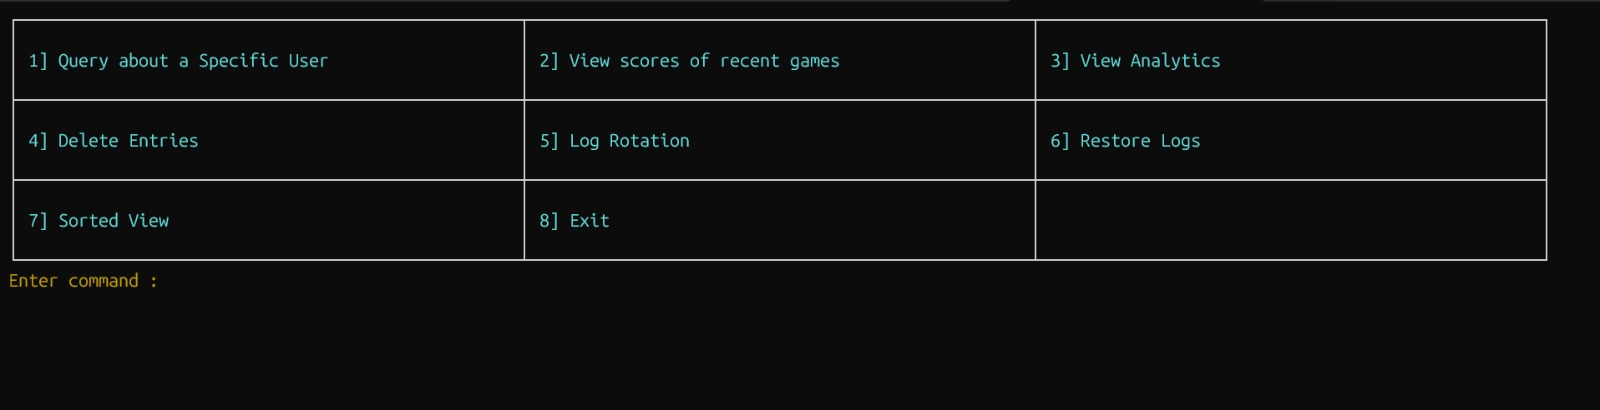
\includegraphics[width=0.8\linewidth]{large_menu.jpg}
            \caption{Menu for all possible Functionalities}
            \label{fig:menu}
        \end{figure}

        \item \underline{User selection} : This can be used to select a specific user to limit the anlaytics and views to the selected user.The username is stored globally and reused across multiple functions. Query selector can also be used to switch to view analytics of all users by entering default command (Enter) in the query selector.

        \item \underline{View Recent Scores} : It used to view the recent game stats from history.txt in a tabular format. Records can be viewed for all users or a specific user.

        \item \underline{Analytics} : It is used to view analysis of game of individual user or the analysis of all users. The analysis includes average score, average time survived , No.of deaths by wall and self biting, fraction of wall deaths and list of records corresponding to the max score in the game. The output is given in a tabulated format. The output can be viewed of entire file or for the games played in a specific time range.

        \begin{figure}[hbtp]
            \centering
            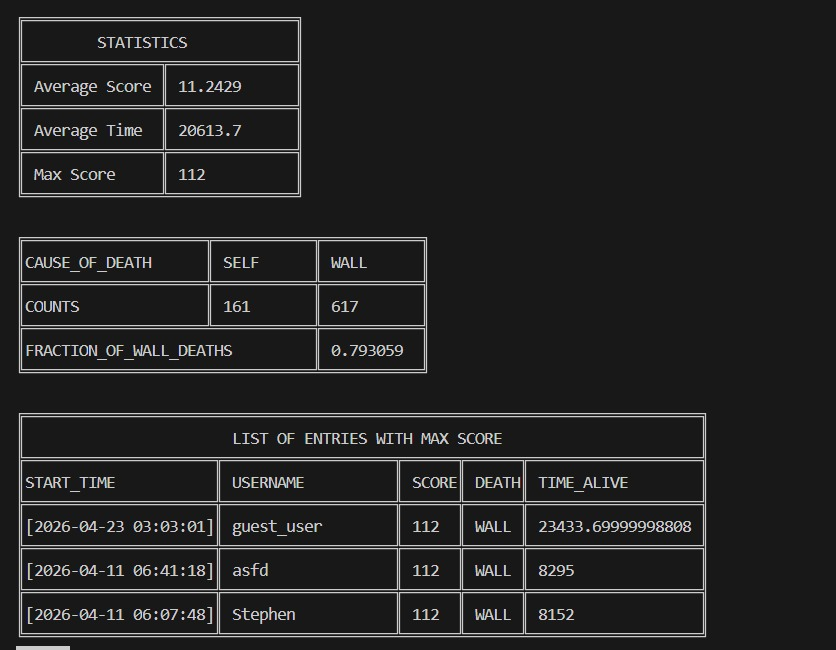
\includegraphics[width=0.8\linewidth]{Analytics.jpg}
            \caption{Analytics of all Users}
            \label{fig:analytics}
        \end{figure}
    
        \item \underline{Delete Entries} : It is used to delete entries from history.txt. The entries can be deleted for a particular user , Entries in a range of timestamp chosen by user or to remove misformatted records in history.txt. It also asks for confirmation before deleting the records.

        \item \underline{Sorted View} : It shows the records of user/users sorted by username (ascending/descending) ,timestamp, time survived or score in a tabular format.

        \item \underline{Log Rotation} : It is used to take backup of history.txt in a folder named backup and keep only last 10 entries(By the time of game played) in history.txt .

        \item \underline{Restore Logs} : This is used to restore history.txt if a backup exist. It can be used in cases like when file is empty, when you want current entries in history.txt along with some additional entries from the last backup, etc ...

        \item \underline{Exit and Default} : User can exit to main menu from any given state by pressing 'q' and from menu by pressing q or invoking exit function. Default command can be invoked in several conditions by pressing "enter" like in entering timestamp or a set default in some functions 

        \item \underline{Update Stats} : after each vital function call, updatestats function is called which updates the stats of all essential variables like user,default start and end time,list of all users and handles the empty history.txt file by calling other functions and taking confirmation from user.

        \item \underline{Tabular and Colored Display} : Almost all outputs are shown in well designed tables in a formatted manner . All warnings , messages ,errors ,success and content are displayed in color code indicating the type of message.  
    \end{enumerate}


    \subsubsection{Advanced Features}
    \begin{enumerate}
        \item \underline{Dynamic Menu Display}  The menu displayed is dynamically adjusted to terminal width allowing proper visibility and access across variable terminals. 

    \begin{figure}[htbp]
     \centering
     % Large terminal
     \begin{subfigure}[b]{0.45\textwidth}
         \centering
         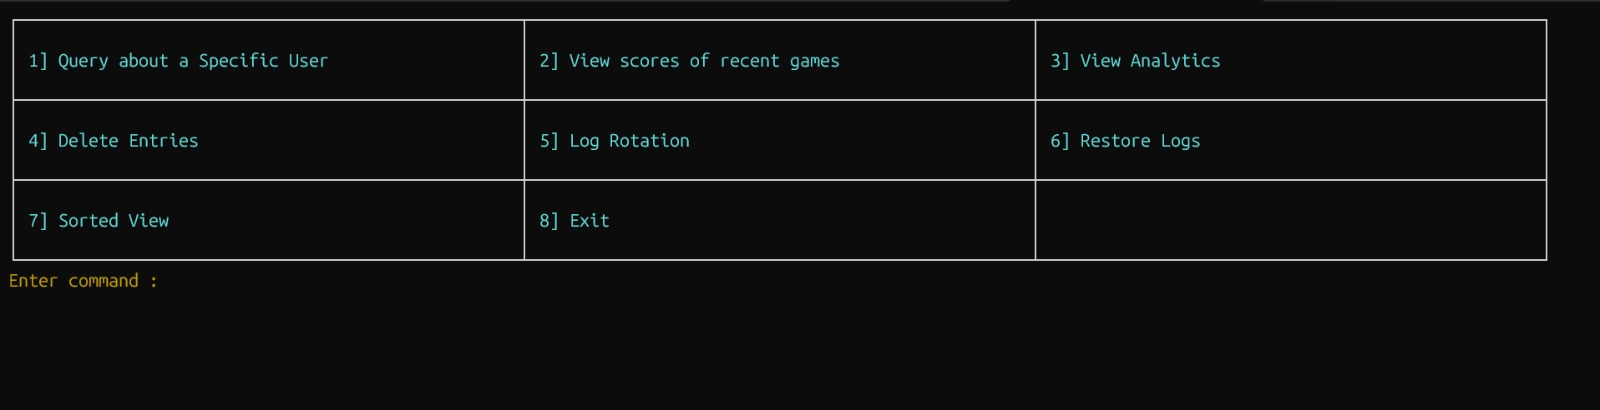
\includegraphics[width=\textwidth]{large_menu.jpg}
         \caption{Menu in Large terminal}
         \label{fig:large_table_display}
     \end{subfigure}
     \hfill % Adds horizontal space between the images
     % Second Subfigure
     \begin{subfigure}[b]{0.45\textwidth}
         \centering
         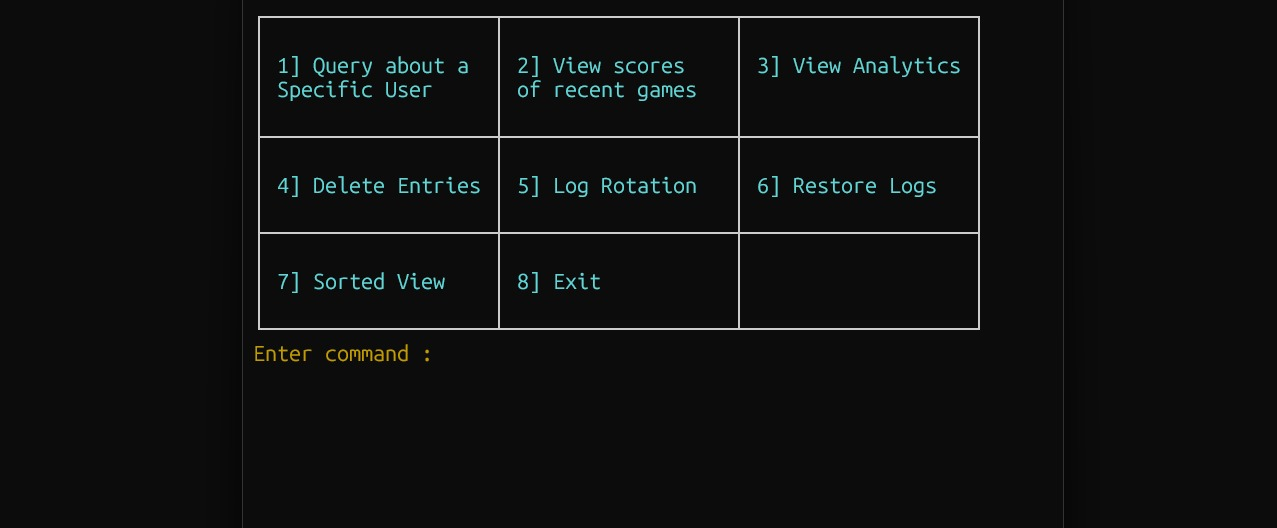
\includegraphics[width=\textwidth]{small_menu.jpg}
         \caption{Menu in Small Terminal}
         \label{fig:small_table_display}
     \end{subfigure}
        
     \caption{Auto adjusted table according to width of the terminal}
     \label{fig:dynamic_table}
    \end{figure}

    \item \underline{User Experience} : To improve user experience , we have added functions like single click selection to instantaneously respond to the command and avoiding classic need of pressing enter key. We have also cleared terminal / some lines in it wherever necessary to avoid cluttering of too many error messages and displaying each new function on a clear terminal. While entering inputs like username or timestamp, we have allowed navigation through all available terminal commands to move to start/end of line , use arrow keys , etc ... .

    \item \underline{Handling Edge Cases} : A keen attention has been payed on edge cases . If you start the script with no history.txt or with misformatted history.txt , either the script will exist with an error message or give you a choice to exit script or view and delete misformatted records from the file . This helps in smooth user experience after the start of the main script.
    \end{enumerate}

    \begin{figure}[H]
     \centering
    
    %  \hfill % Adds horizontal space between the images
     % Second Subfigure
     \begin{subfigure}[b]{0.45\textwidth}
         \centering
         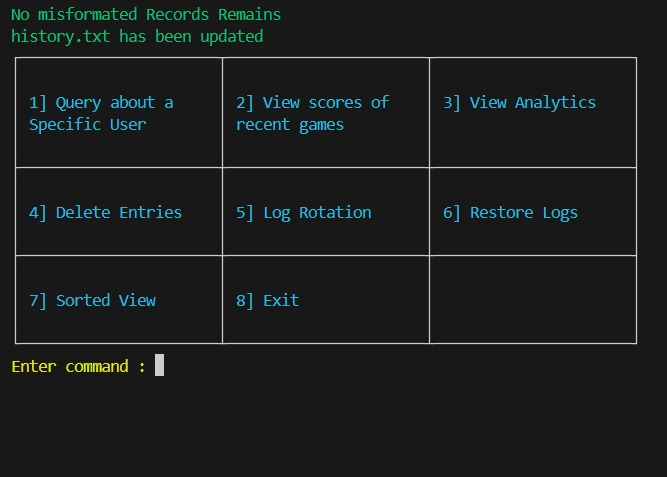
\includegraphics[width=\textwidth]{user_experience_1.jpg}
         \caption{Interactive User Experience}
         \label{fig:user_experience}
     \end{subfigure}

     \begin{subfigure}[b]{0.45\textwidth}
         \centering
         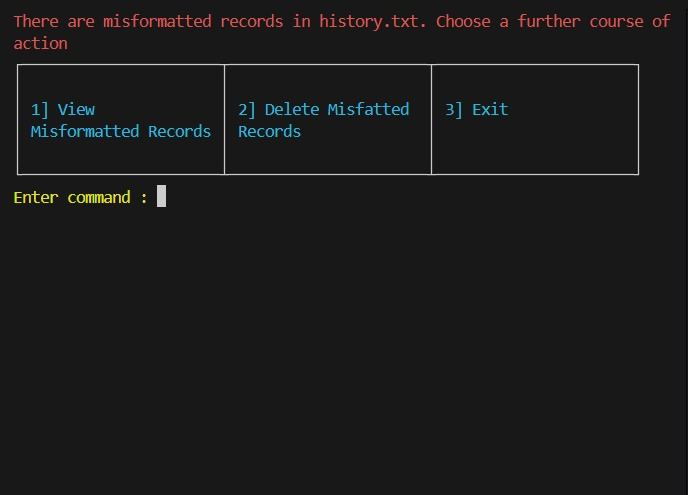
\includegraphics[width=\textwidth]{misformatted.jpg}
         \caption{Misformatted Records in history.txt}
         \label{fig:misformatted}
     \end{subfigure}
     \hfill % Adds horizontal space between the images
     \caption{Edge Cases and User Experience}
     \label{fig:edge_case}
    \end{figure}

\section{Design and Architecture}

The project follows a three-layer architecture consisting of a frontend gameplay layer, a backend persistence layer, and an administration layer. This separation ensures that gameplay logic, record storage, and system management remain independent from each other. Each layer is responsible for a specific task, which improves maintainability and makes debugging much easier.

\subsection{Frontend Layer}

The frontend is responsible for the real-time gameplay experience and user interaction. It is built using HTML, CSS, JavaScript, HTML5 Canvas, and Bootstrap 5. The HTML structure separates the interface into the main game canvas, left-side information cards, game-window, and multiple modal windows such as the start modal, rules modal, death modal, and statistics modal. Bootstrap is mainly used for modal management and responsive layout support.

In script.js, the game's state is controlled using the \texttt{GameState} class, while player-specific information is handled using the \texttt{User} class and snake properties are managed through the \texttt{Snake} class. The code separates logical updates to the game state and graphical rendering onto the canvas into different functions. The function \texttt{updateState()} updates movement, collision checks, fruit consumption, and death conditions at fixed game ticks, while \texttt{updateCanvas()} handles only drawing operations on the canvas. This prevents rendering code from interfering with game logic and improves code clarity. Both of these functions and an \texttt{updateUI()} function are repeatedly called within a \texttt{gameLoop()} function using the \texttt{requestAnimationFrame} function, managing their respective calling intervals by storing the time of last call and calculating current time using \texttt{performance.now()}.

The frontend also preloads all required sprite images before gameplay begins, reducing lag and unnecessary loading during rendering.

\subsection{Backend Layer}

The backend is implemented using Python and Flask and is designed mainly for serving the web page and validation of game records. It serves the main webpage on localhost and exposes the \texttt{/save\_score} route which accepts POST requests from the frontend whenever a game ends. After successful validation of a received record, it is appended to \texttt{history.txt}.

\subsection{Administration Layer}
The administration layer is implemented as a Bash-based TUI for handling stored game records. Instead of using a database system, the project uses plaintext history storage and standard shell utilities such as \texttt{awk}, \texttt{grep}, \texttt{sort}, \texttt{cut}, \texttt{fold}, and \texttt{date}. This makes the system lightweight, portable, and easy to inspect manually.

The Bash script is designed around reusable validation functions, formatted table output functions, and separate feature functions for analytics, deletion, sorting, log rotation, and restore operations. Dynamic ASCII table generation is used to display records cleanly inside the terminal. Timestamp filtering and validation are handled carefully to prevent invalid ranges or malformed records from causing failures.

The admin panel also checks for misformatted records during startup and forces correction before continuing. This protects later operations such as analytics and deletion from unexpected file structure issues.

\subsection{Layer Communication}

The three layers communicate using a shared pipeline centered around \texttt{history.txt}.

The frontend sends the latest game record to the backend using Fetch API and a POST request to the Flask route \texttt{/save\_score}. The backend validates the record and writes it into \texttt{history.txt}. The Bash admin panel then reads the same file to generate analytics, recent score views, sorting operations, deletion tools, backup creation, and restore functionality.

\subsection{Choice of history.txt Format}

The file \texttt{history.txt} stores one game record per line using a CSV-style format:

\texttt{[start\_time],username,score,cause,time\_alive}

An example record is:

\texttt{[2026-04-11 05:28:19],guest\_user,3,WALL,26.200}

This format was chosen because it is human-readable, and works naturally with Bash, especially \texttt{sort} and \texttt{date} commands for which this date format is natural. This format is easily accessible by tools like \texttt{awk}, \texttt{sort}, and \texttt{grep} to operate efficiently and perform the required operations. Comma can be chosen as a delimiter because no data field here will normally have a comma inside it. (Ensured by python before saving).

\section{Directory structure}
\begin{itemize}
    \item \texttt{admin.sh}: Bash-based admin TUI used for analytics, sorting, deletion, log rotation and restoring logs.
    \item \texttt{app.py}: Flask backend server responsible for serving the web page, validating incoming records, and saving them into \texttt{history.txt}.
    \item \texttt{history.txt} (formed after running the game): Plaintext CSV-style file storing all game records including timestamp, username, score, cause of death, and survival time.
    \item \texttt{requirements.txt}: Contains Python dependencies required to run the backend server.
    \item \texttt{README.md}: Basic project overview containing setup instructions and project description.
    \item \texttt{.gitignore}: Specifies files and folders excluded from Git version control.
    \item \texttt{report.tex}: Main \LaTeX  file used to write the project report.
    % \item \texttt{report.bib}: Bibliography file containing references used in the report.
    \item \texttt{Makefile}: Makefile to compile the Latex files into the final report PDF.
    \item \texttt{report.pdf}: Compiled final PDF version of the project report.
    \item \texttt{report\_images/}: Folder containing images included in report.pdf
    \item \texttt{templates/index.html}: Main HTML structure of the Snake Game user interface including canvas, cards, and modals.
    \item \texttt{static/css/bootstrap.min.css}: Minified Bootstrap CSS library used for responsive layout and modal styling.
    \item \texttt{static/css/styles.css}: Custom CSS file containing neobrutalist UI styling, animations, and responsive design rules.
    \item \texttt{static/js/bootstrap.bundle.min.js}: Minified Bootstrap JavaScript library for modal and UI component functionality.
    \item \texttt{static/js/data.js}: Auto-generated JavaScript file containing sprite image paths used for preloading assets.
    \item \texttt{static/js/script.js}: Main JavaScript file containing game logic, rendering, input handling, collision checks, fruit effects, and UI updates.
    \item \texttt{static/fonts/Squada\_One/}: Directory containing the custom font files used in the UI.
    \item \texttt{static/media/sprites/}: Stores snake sprites for different themes and fruit images used during gameplay.
    \item \texttt{static/media/ui/}: Contains icons and decorative UI assets used in modals and info cards.
    \item \texttt{static/media/sounds/}: Stores sound effects and audio assets used during gameplay.
\end{itemize}

\section{Installation and Setup}

To run the project, first clone the repository and move into the project directory.

\begin{verbatim}
git clone https://github.com/Vasu-Vijay/snake-game-ssl.git
cd snake-game-ssl
\end{verbatim}

It is recommended to create and activate a Python virtual environment before installing dependencies.

\begin{verbatim}
python3 -m venv venv
source venv/bin/activate
\end{verbatim}

Install the required Python packages using \texttt{requirements.txt}.

\begin{verbatim}
pip install -r requirements.txt
\end{verbatim}

The backend server can then be started using:

\begin{verbatim}
python3 app.py
\end{verbatim}

This serves the web application locally at:

\begin{verbatim}
http://127.0.0.1:5000
\end{verbatim}

The Bash admin panel can be launched separately using:

\begin{verbatim}
bash admin.sh
\end{verbatim}

Note: The admin panel requires \texttt{history.txt} to be present in the project root directory with the correct header format (this file is auto-generated when you play your first game). If the file is missing or incorrectly formatted, the script exits with an error.

\section{Usage}

\subsection{Running the Web Game}

After starting the Flask server using \texttt{python3 app.py}, open any browser on your device and visit \texttt{http://127.0.0.1:5000}. The start modal appears automatically when the page loads.

The user first enters a username, selects the preferred graphics mode, and may view the rules using the Rules button. Pressing the Start Game button (or directly pressing Enter) initializes the game and opens the main gameplay interface.

\begin{figure}[H]
    \centering
    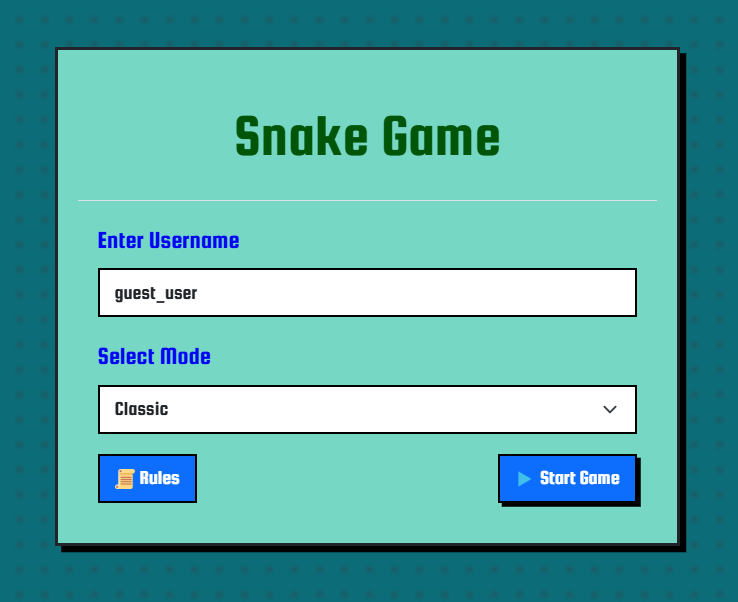
\includegraphics[width=0.75\linewidth]{startmodal.png}
    \caption{Start Modal shown on page load}
\end{figure}

\subsection{Playing the Game}

The snake is controlled using either the Arrow keys or the WASD keys. The objective is to collect fruits, increase score, and survive as long as possible while avoiding collisions with walls and the snake's own body.

Different fruits provide different effects. Carrot increases score by 1, Triple Carrot increases score by 3, Golden Apple grants temporary immunity, and Speed-Up Fruit temporarily increases movement speed and increases score by 1.

During gameplay, the left-side information cards display score, snake length, high score, survival time, and active power-up durations using progress bars.

\begin{figure}[H]
    \centering
    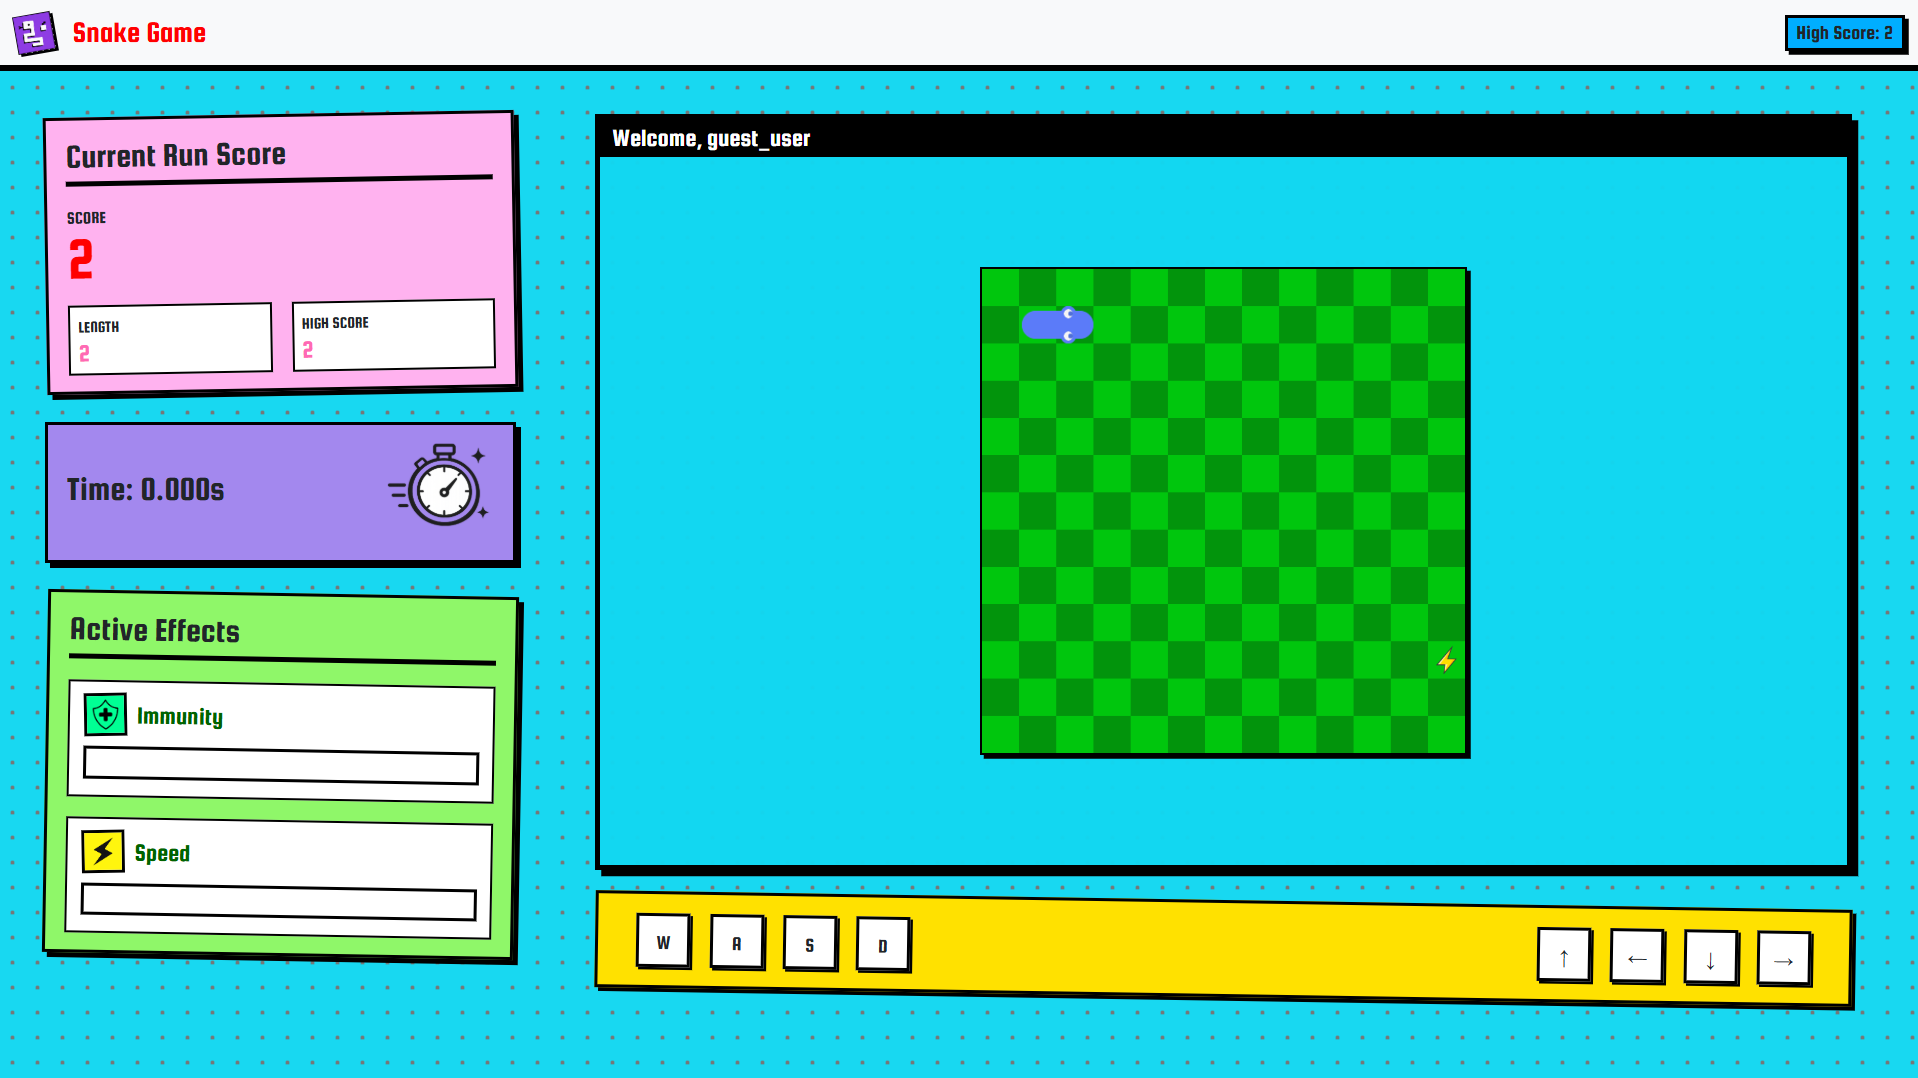
\includegraphics[width=0.85\linewidth]{maingame.png}
    \caption{Main Gameplay Interface}
\end{figure}

The interface is also responsive across different screen sizes and aspect ratios. Bootstrap layout utilities and custom CSS ensure that the canvas, side panels, cards, and controls resize properly without breaking the layout or affecting gameplay.

\begin{figure}[H]
    \centering
    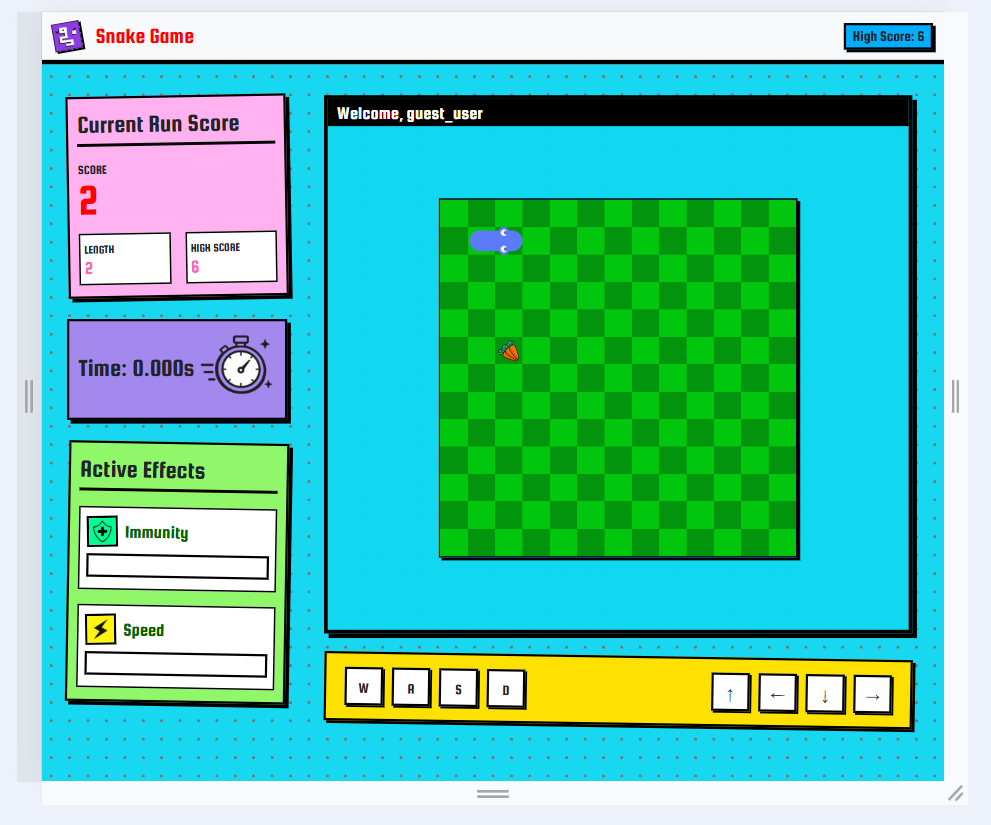
\includegraphics[width=0.75\linewidth]{smallgame.png}
    \caption{Responsive layout under a different screen aspect ratio}
\end{figure}

\subsection{Game Over and Statistics}

When the snake dies, the Game Over modal appears showing the cause of death, final score, survival time, and the current high score.

The Retry button allows the player to restart quickly without entering the username again.

\begin{figure}[H]
    \centering
    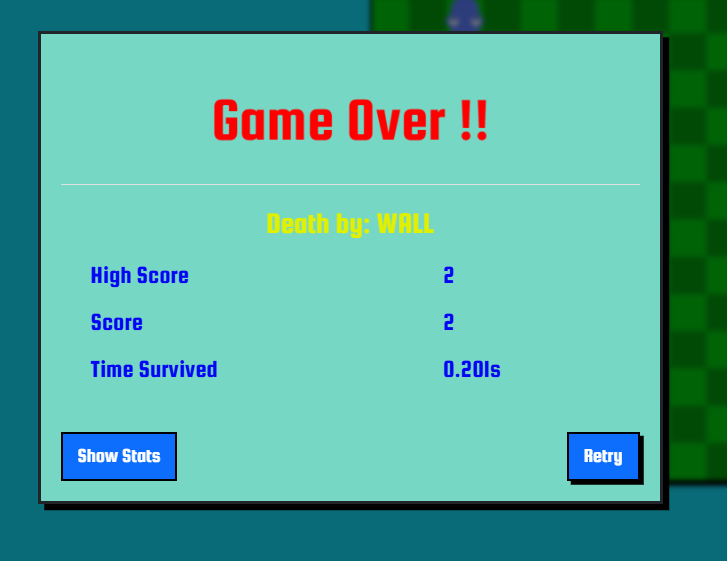
\includegraphics[width=0.65\linewidth]{gameover.png}
    \caption{Game Over Modal}
\end{figure}

The Show Stats button opens the statistics modal, which displays all game runs from the current session in a scrollable table.

After every completed run, the latest game record is automatically sent to the backend and stored in \texttt{history.txt}.

\begin{figure}[h]
    \centering
    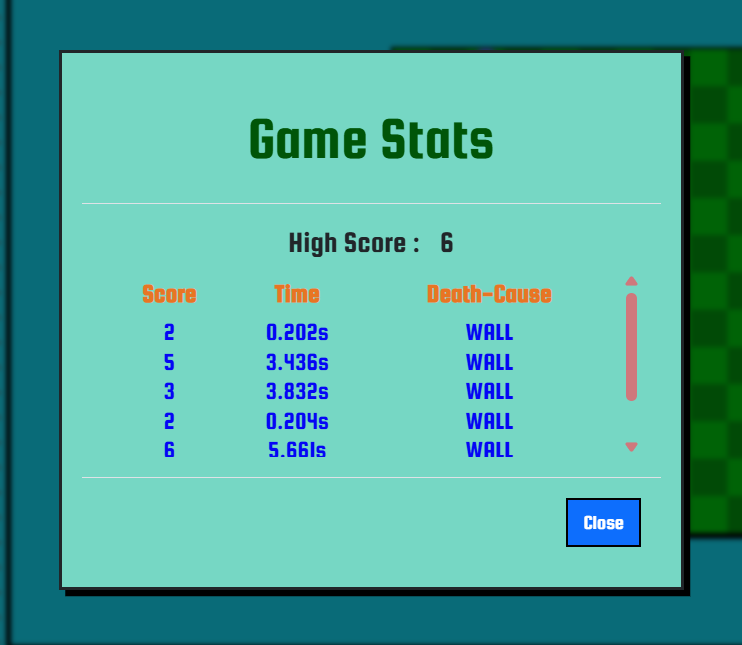
\includegraphics[width=0.65\linewidth]{statsmodal.png}
    \caption{Statistics Modal}
\end{figure}

\subsection{Using the Admin Panel}

The Bash admin panel can be started separately using:

\begin{verbatim}
bash admin.sh
\end{verbatim}

The terminal menu provides options such as querying a specific user, viewing recent scores, analytics generation, sorted views, deleting entries, log rotation, and restoring backup logs.

All operations are performed directly on \texttt{history.txt}, making the admin panel the main tool for long-term record management and maintenance.

\section{Project Journey}
    \subsection{Journey}
        \begin{enumerate}
            \item Learned using Various tools like Bootstrap and CSS for designing dynamic web page
            \item Modularizing code for reusage, avoiding cluster and easy debugging
            \item Learned Hosting Server by using Flask library of Python
            \item Using developer tools in browser for quick debug and website interaction
            \item Learnt the need of very keen attention while coding especially in languages like bash
            \item Learnt Exploring documentation to know about multiple commands/features which help in executing desired functionality.
            
        \end{enumerate}
    \subsection{Hurdles}
        \begin{enumerate}
    \item \textbf{Handling ANSI Escape Sequences}: When using the \texttt{read -p} command with colored prompts (e.g., \texttt{\textbackslash e[32m} for green text), the Bash shell mistakenly includes the length of the escape sequence in its terminal width calculation. Since these characters do not occupy physical space, this miscalculation causes the prompt to overwrite itself or wrap incorrectly when the terminal is resized. To resolve this, we wrapped all non-printing escape sequences between \texttt{\textbackslash 001} (Start of Header) and \texttt{\textbackslash 002} (Start of Text) markers. These markers signal to the \texttt{readline} library that the enclosed text has zero width, ensuring accurate cursor positioning.

    \item \textbf{Dynamic Menu Display} : This took a lot of efforts and deep research to dynamically calculate terminal width and do folding according to no.of columns and column width in table.

    \item \textbf{Handling Edge Cases} : Handling Edge cases took a lot of efforts as many errors came when testing username validation and history.txt validation.

    \item \textbf{Syntax} : Many Errors came due to the strict syntax of bash. It was many times difficult to identify the source of error as many errors were unnoticable.
\end{enumerate}

    
\section{What we would do with ten more hours}
Ten more Hours for our project would have been used for:
    \begin{itemize}
        \item Improving Display of contents in bash.
        \item Introducing new features and fruits in snake game.
        \item Introducing new functions to avoid repetition of code.
        \item Making UI interface more better by adding more animations.
    \end{itemize}

%%%%%%%%%%%%%%%%%%%%%%%%%%%%%%%%%%%%%%%%%%%%%%%%%%%%%%%%%%%%%%%%%%%%%%%%%%%%%
% \printbibliography(optional!!!!!!!!!)

\end{document}